% ============================================================
% f2013_shanghai_arts_q19_pyramid.tex
% 2013 上海卷（文科）第 19 题 正三棱锥 O-ABC（TikZ 矢量重绘）
% 几何：底面为边长为 2 的正三角形 ABC，顶点 O 在底面上的射影为底面中心，
%       高为 1。AB 为被遮挡的底面棱，画虚线；其余各棱实线。
% ============================================================
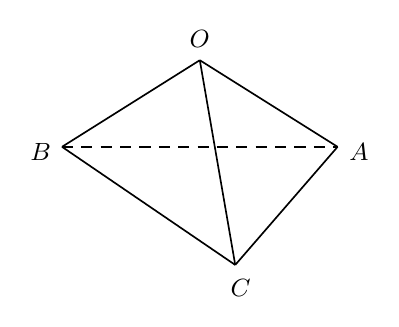
\begin{tikzpicture}[
  x=1cm, y=1cm,
  every node/.style={font=\small, inner sep=1pt},
  line/.style={line width=0.6pt},
  hidden/.style={line width=0.6pt, dash pattern=on 4pt off 3pt},
]

  \coordinate (O) at (0,3.05);
  \coordinate (B) at (-1.75,1.95);
  \coordinate (A) at (1.75,1.95);
  \coordinate (C) at (0.45,0.45);

  % 侧棱
  \draw[line] (O) -- (A);
  \draw[line] (O) -- (B);
  \draw[line] (O) -- (C);

  % 底面棱：AB 被遮挡
  \draw[hidden] (B) -- (A);
  \draw[line] (B) -- (C);
  \draw[line] (C) -- (A);

  % 标签
  \node at (0,3.32) {$O$};
  \node at (-2.02,1.88) {$B$};
  \node at (2.02,1.88) {$A$};
  \node at (0.52,0.16) {$C$};

\end{tikzpicture}
